\documentclass[conference]{IEEEtran}

\usepackage{cite}
\usepackage{amsmath,amssymb,amsfonts}
\usepackage{algorithmic}
\usepackage{graphicx}

\usepackage{subfigure}
\usepackage{textcomp}
\usepackage{xcolor}
\def\BibTeX{{\rm B\kern-.05em{\sc i\kern-.025em b}\kern-.08em
    T\kern-.1667em\lower.7ex\hbox{E}\kern-.125emX}}
\begin{document}

\title{Predicting Next Day Stock Price by using Supervised Machine Learning Models on Technical Indicators\\
}

\author{\IEEEauthorblockN{Man Yi Yeung}
\IEEEauthorblockA{\textit{College of Engineering} \\
\textit{Drexel University)}\\
Philadelphia, PA, United States \\
my442@drexel.edu}
}

\maketitle

\begin{abstract}
This project focuses on next-day stock price prediction by applying machine learning models on 27 technical indicators of the past 5 days. The stocks that were investigated are IBM, Apple (AAPL) and Johnson and Johnson (JNJ). Stock price and technical indicator data for the past 20 years are used to train the models after k-fold cross-validation split with blocking, normalization with standard scaler or min max scaler, as well as principle component analysis for dimensionality reduction. The machine learning models that were tested are linear regression, Bayesian ridge regression, lasso regression, decision tree regression, random forest regression, support vector regression, and long short term memory. From measuring the root mean square error (RMSE) of the prediction with the actual stock price for the IBM stock, the best models are the long short term memory model, linear regression and Bayesian ridge regression, with a RMSE score of around 2 to 5 for all price types of the IBM and JNJ stocks. The models work well for these two of the three stocks tested. For AAPL, this approach produces high RMSE values of more than 120, suggesting this stock's price trend does not have strong correlation with the exact past technical indicator combination chosen for this analysis. Thus, this technical indicator approach is not a generalized approach for all stocks, and may require adjustments for some stocks.
\end{abstract}

\section{Introduction}
The stock market is a significant part of the economy. Individuals, companies, and governments can influence and are impacted by changes in the stock market. Predicting stock price is a popular topic in machine learning. Stock investment strategies are very complex problems because it involves large amounts of data, and stock price movements are influenced by many factors from the the performance of the company, to the well-beings of related industries, and to the current situation of the government. Many research has been done in this area, and this project aims to predict the daily stock prices for three companies by using past technical indicators data gathered through Alpha Vantage API.

There are two main methods utilized in stock market prediction. The first one is fundamental analysis, where the stock price is compared to the actual worth of the company's stock. The estimated intrinsic value of the stock is based on the financial performance, company's business goals and so on. This approach is mainly used in long term stock prediction. The second approach is the technical analysis, where short term price trends are predicted from analyzing past pricing data and past technical indicator to evaluate price signals. Technical analysis is the approach used in this project, where past technical indicators data are used to predict the next day stock price.

\section{Related Work}

There are many past research conducted in the area of stock price prediction. The approach and the machine learning models used differ as new prediction tools and concepts emerge.

One of the approach is artificial neural networks (ANN), a paper is published in 2004, using univariate neural networks approach to provide short term stock market predictions in order to evaluate profitability of different trading signals for S\&P 500 stocks in the years from 1965 to 1999 \cite{b1}. Another study uses least squares support vector machine (LSSVM) method to predict stock market trend based on historical stock data \cite{b2}. This method evolves the input features through evolutionary algorithms or more specifically genetic algorithm. The genetic algorithm mimics Darwin's natural selection process in order to evolve inputted features to provide optimize prediction.

A term called "Stock2Vec" has been used to describe many algorithms that predicts stock price using different kinds of information of the stock market. One usage of this term is as a trained word embedding in a two-stream gated recurrent unit network approach to conduct sentiment analysis on financial news in order to stock price in the short run \cite{b3}. Another study uses "Stock2Vec" to represent the individual stock rather than word embedding. In this study, the embedding is trained as features and used with temporal convolutional network and deep learning in order to predict daily stock prices \cite{b4}.

Past work that is similar to this project's approach includes a study of logistic regression using over 270 features of qualitative and quantitative information about the stock to predict the stock price trend as a classification problem of whether the stock is moving up, down or stationary \cite{b5}. There is also a similar paper, where artificial neural network (ANN), support vector machine (SVM), random forest and naive-Bayes are use on technical parameters calculated using stock trading data of open, high, low and close price, in order to predict stock price in the Indian market \cite{b6}.


\section{Methodology}
The project is completed using python 3.7.9 with Jupyter Notebook. It utilizes pandas, numpy, matplotlib libraries for data processing and plotting. Sklearn, Keras and TensorFlow are used for different implementing machine learning models. 

Figure \ref{figure:flow_chart1} shows a general flow chart of how the stock price and technical indicators data are pre-processed and fed to different machine learning models for price prediction.

\begin{figure}
  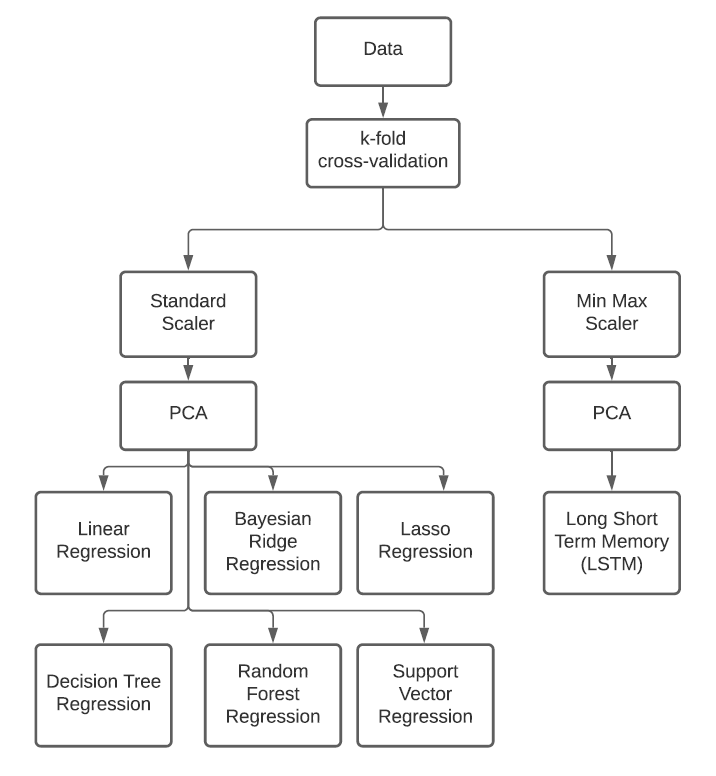
\includegraphics[width=\linewidth]{./image/flow_chart.PNG}
  \caption{Flow Chart of Machine Learning Process}
  \label{figure:flow_chart1}
\end{figure}

\subsection{Data Collection}\label{AA}
Stock pricing and technical indicators data are collected from Alpha Vantage API. The four types of daily stock price, open, close, high, and low, are the dependent variables of the analysis. The open and close price refers to the first and last bid price of the day, while the high and low price corresponds to the maximum and minimum price on a particular day. 

The independent variables are the technical indicators over the past 5 days. There are a total of 27 technical indicators used including the volume of trade, dividend, simple moving average (SMA), exponential moving average (EMA), moving average convergence/divergence (MACD), stochastic oscillator (STOCH), relative strength index (RSI), average directional movement index (ADX), commodity channel index (CCI), Aroon indicator (AROON), Bollinger bands (BBANDS), Chaikin A/D line (AD), and on balance volume (OBV). (Note: Some of these indicators may contain multiple values all taken into account in the dependent variable dataset.) These specific features are chosen because of their popularity and being marked with "high usage" on Alpha Vantage API's website. For some indicators, the number of data points used to calculate values such as moving averages need to be specified. Two values, 10 and 20 data points, are chosen to provide a better general picture for the next day stock price prediction. 


\subsection{Data Pre-processing}
There are three main steps in the pre-processing of the data, k-fold cross validation, data scaling, and principle component analysis (PCA).

\subsubsection{K-Fold Cross-Validation}

The first step is k-fold cross-validation. The reason of employing k-fold cross-validation instead of the normal train-test split is that the sample size with almost 20 years of data is very large, and it allows for models to be tested over different time range. Two types of k-fold cross-validation are used. One is the normal k-fold cross-validation for time-series data without shuffling and blocking. The second type has has blocking, which means only historical data up to some point is used to train the model, not all data prior to the train-test split. The difference between the two approaches can be visualized in Figure \ref{figure:k_fold_blocking_no_blocking}. In the pre-processing step of the data, a k values or the number of splits of 10 is used, but Figure \ref{figure:k_fold_blocking_no_blocking}, k value of 5 is used for easier visualization purpose.


\begin{figure}
	\hfill
	\subfigure[k Fold Without Blocking]{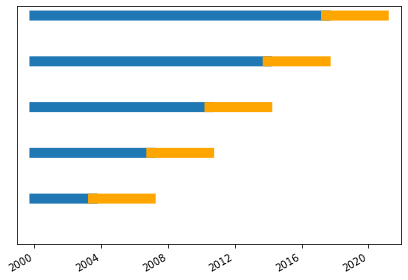
\includegraphics[width=0.45\linewidth]{./image/k_fold_no_blocking.PNG}}
	\hfill
	\subfigure[k Fold With Blocking]{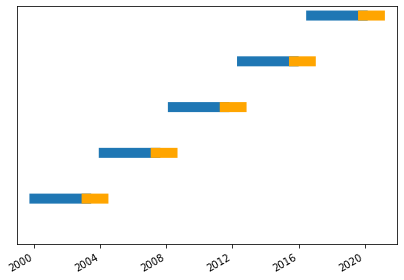
\includegraphics[width=0.45\linewidth]{./image/k_fold_blocking.PNG}}
	\hfill
	\caption{k Fold Time Series Split Without Blocking (on the left) and With Blocking (on the right), with k value = 5}
	\label{figure:k_fold_blocking_no_blocking}
\end{figure}

\subsubsection{Data Scaling}
The second stage is scaling or standardization. As shown in Figure \ref{figure:flow_chart1}, the two types of scaling method used are standard scaler and min max scaler. Standard scaler enable the standardized value to have a mean of 0 and a standard deviation of 1. The min max scaler transform the data to have values between 0 and 1 only.

\subsubsection{Principle Component Analysis}
The last step before model implementation is Principle Component Analysis or PCA, aimed to reduce the dimensionality of the independent variable dataset. By performing PCA, the size of the dataset can be reduced, while preserving most of the information expressed by the original features. The extent of this reduction is determined by setting the amount of variance of the original features that the reduced dataset needs to explain. This threshold is set to 95$\%$. The effects of PCA on the performance of various regression models used and the Long Short Term Memory model are studied, and the results are presented in the section IV. Experiments and Results \ref{section:experiments}.


\subsection{Implementation of Supervised Machine Learning Models}
Seven different supervised machine learning models are trained with pre-processed data to predict the next day stock price. They are linear regression, Bayesian ridge regression, lasso regression, decision tree regression, random forest regression, support vector regression, and long short term memory. They are all regression models except for long short term memory, which is a neural network model. The performances of each model are evaluated by calculating the root mean square error (RMSE) values between the actual historical stock price data and the model prediction.

\section{Experiments and Results}
\label{section:experiments}
The prediction on next day stock price was performed on three stocks for IBM, Apple ('AAPL') and Johnson and Johnson ('JNJ'). All four types of daily stock price, daily open, daily close, daily high, and daily low are forecasted for each company's stock. 

For the results in the following sections, the price predictions and RMSE values are given for the IBM stock and for daily open price, unless explicitly written otherwise. The difference in predictions and RMSE values for the four price types are very small, and comparison among price types are shown in \ref{subsection:forecast result}. 

\subsection{Impact of k-fold Cross Validation with and without Blocking on Forecast Performance}
For the "IBM" stock, the impact of whether to have k-fold cross-validation with or without blocking is studied with a k value of 10. The model prediction RMSE values for with and without blocking are presented in Figure \ref{figure:RMSE_blocking_no_blocking}. 

\begin{figure}
	\subfigure[RMSEs of k Fold Without Blocking]{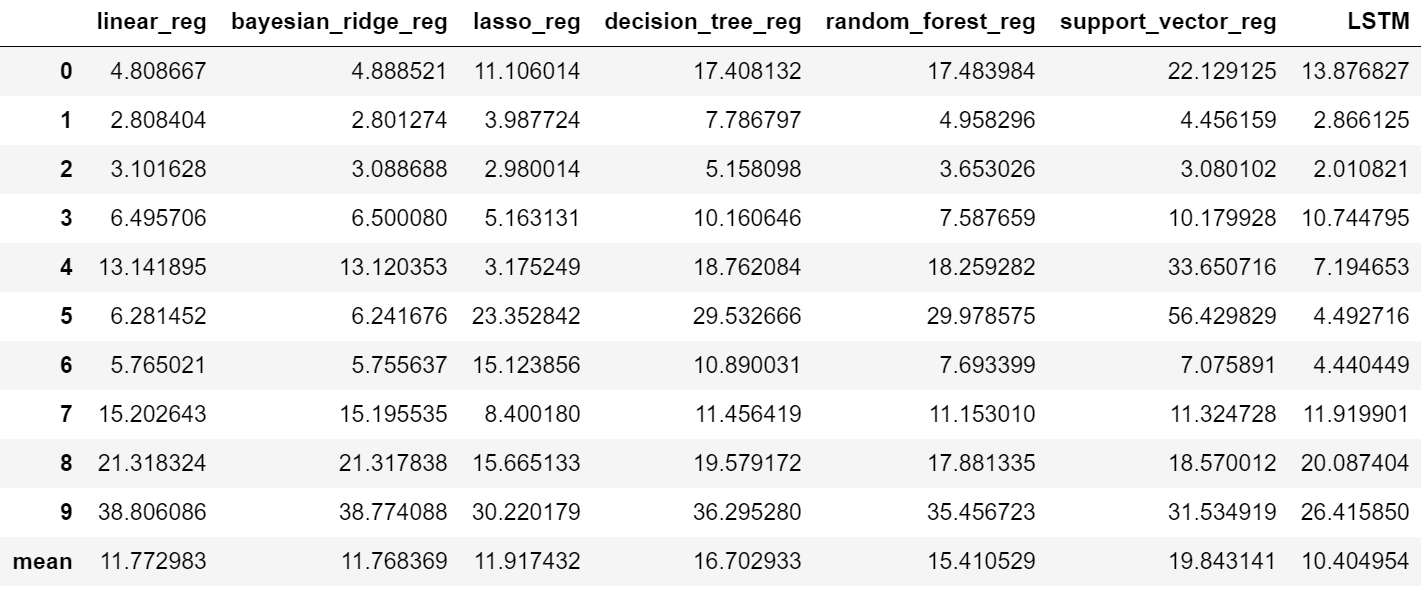
\includegraphics[width=\linewidth]{./image/k_fold_IBM_RMSE_no_blocking.PNG}}
	\subfigure[RMSEs of k Fold With Blocking]{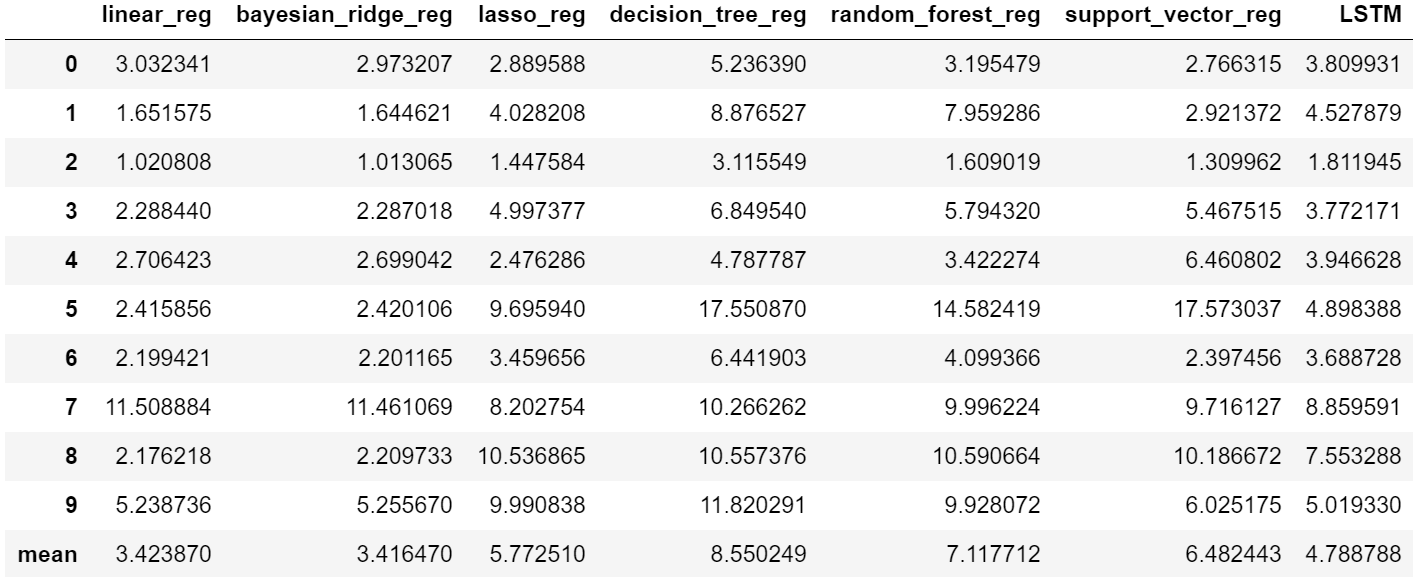
\includegraphics[width=\linewidth]{./image/k_fold_IBM_RMSE_blocking.PNG}}
	\caption{RMSE values for predictions of various machine learning models on k Fold Time Series Split Without Blocking data (on the top) and on With Blocking data (on the bottom)}
	\label{figure:RMSE_blocking_no_blocking}
\end{figure}

In Figure \ref{figure:RMSE_blocking_no_blocking}, k-fold cross validation with blocking results in mean RMSE values of between 3 and 10 for each model and a maximum RMSE of no more than 18. For result obtained without blocking k-fold cross validation, the mean RMSE values range between 10 and 20, with a maximum at more than 38. From this experiment, it can be observed that k-fold cross-validation with blocking will generate a better forecast. 

The RMSE values for the different splits from k-fold cross-validation with blocking are shown in Figure  \ref{figure:RMSE_blocking_no_blocking}-a. In general, the performance of the models are quite consistent despite some peaks at k=5 and k=7 values for certain models. 

\subsection{Impact of Principle Component Analysis on Forecast Performance}

The effects of PCA on model prediction's RMSE scores are shown in Figure \ref{figure:pca_no_pca}. The figure contains the RMSE values of the last split of the k-fold train-test set for IBM's daily open price prediction. For some models, like Bayesian Ridge Regression and Support Vector Regression, there is minimal difference in RMSEs of the predicted results. For other models, the difference is more noticeable, with linear regression having the most different of about 5 in terms of RMSE values. For most models, PCA perform better, except for Bayesian ridge regression, and decision tree regression. 

\begin{figure}
  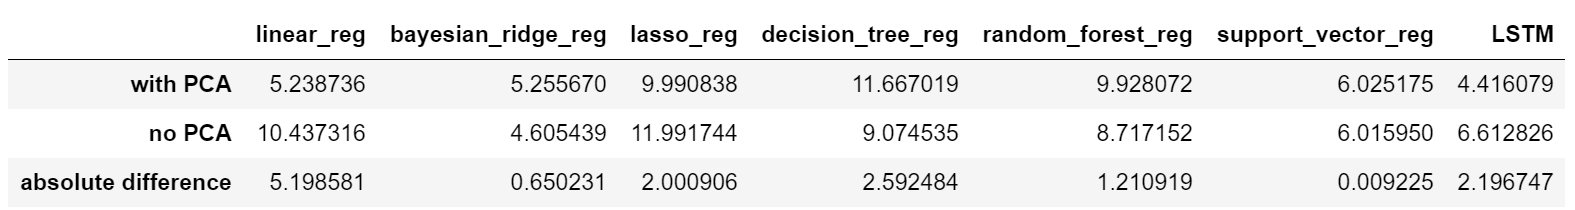
\includegraphics[width=\linewidth]{./image/pca_no_pca.PNG}
  \caption{Comparison of RMSE values for prediction using PCA and without using PCA before apply machine learning models}
  \label{figure:pca_no_pca}
\end{figure}

\subsection{Forecast Result}
\label{subsection:forecast result}
The RMSEs results of the predictions are presented in Figure \ref{figure:RMSE_forecast_result}. Amongst all models, LSTM shows the smallest RMSEs overall at around 3 to 5 for IBM. For regression models, linear regression and Bayesian ridge regression show smaller RMSEs at around 5 for IBM. For the JNJ stock, the RMSEs values are even smaller for all model types. However, for AAPL stock, the performance is much worse than the other two. Random forest regression and support vector regression works better for AAPL, but all models have RMSE values of more than 120. This might be due to inconsistency in technical indicator data or large fluctuations in stock price that the models do not account for. To investigate further, Figure \ref{figure:AAPL_special_rmse} shows the effects for each data split. The models work consistently worse than the other two stocks except for the 0th and the 1st split, which indicates that the cause is movement in stock price for the AAPL are not accounted for in these model, and might not be correlated with past technical indicators.

\begin{figure}
	\subfigure[IBM]{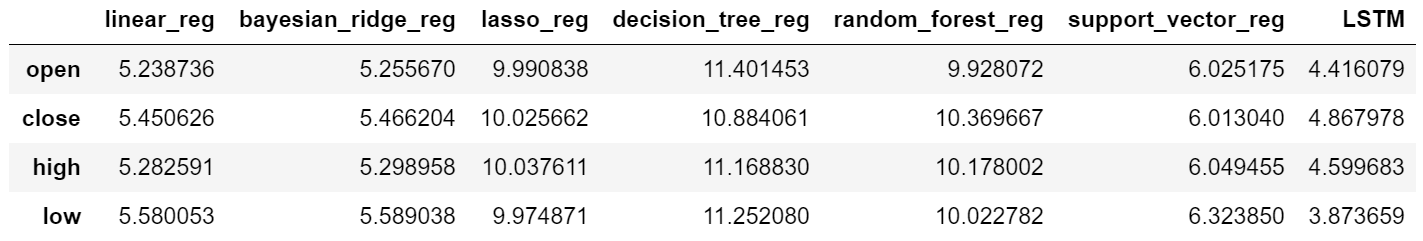
\includegraphics[width=\linewidth]{./image/final_rmse_IBM.PNG}}
	\subfigure[AAPL]{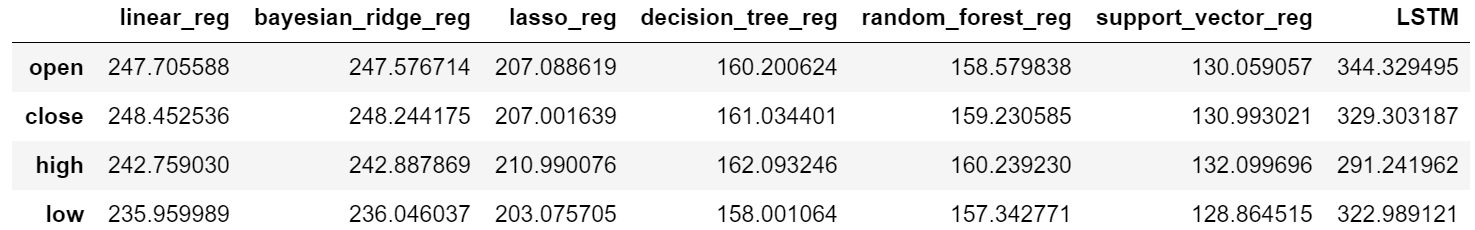
\includegraphics[width=\linewidth]{./image/final_rmse_AAPL.PNG}}
	\subfigure[JNJ]{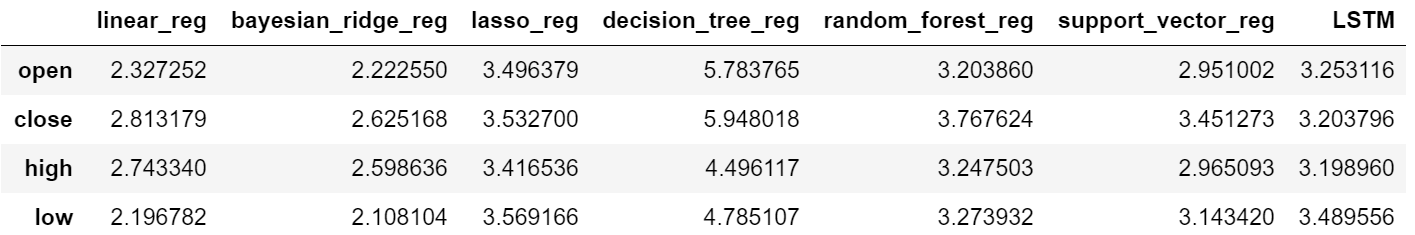
\includegraphics[width=\linewidth]{./image/final_rmse_JNJ.PNG}}
	\caption{RMSE values for IBM, AAPL, and JNJ stocks' daily open, daily close, daily high, and daily low prices}
	\label{figure:RMSE_forecast_result}
\end{figure}

\begin{figure}
	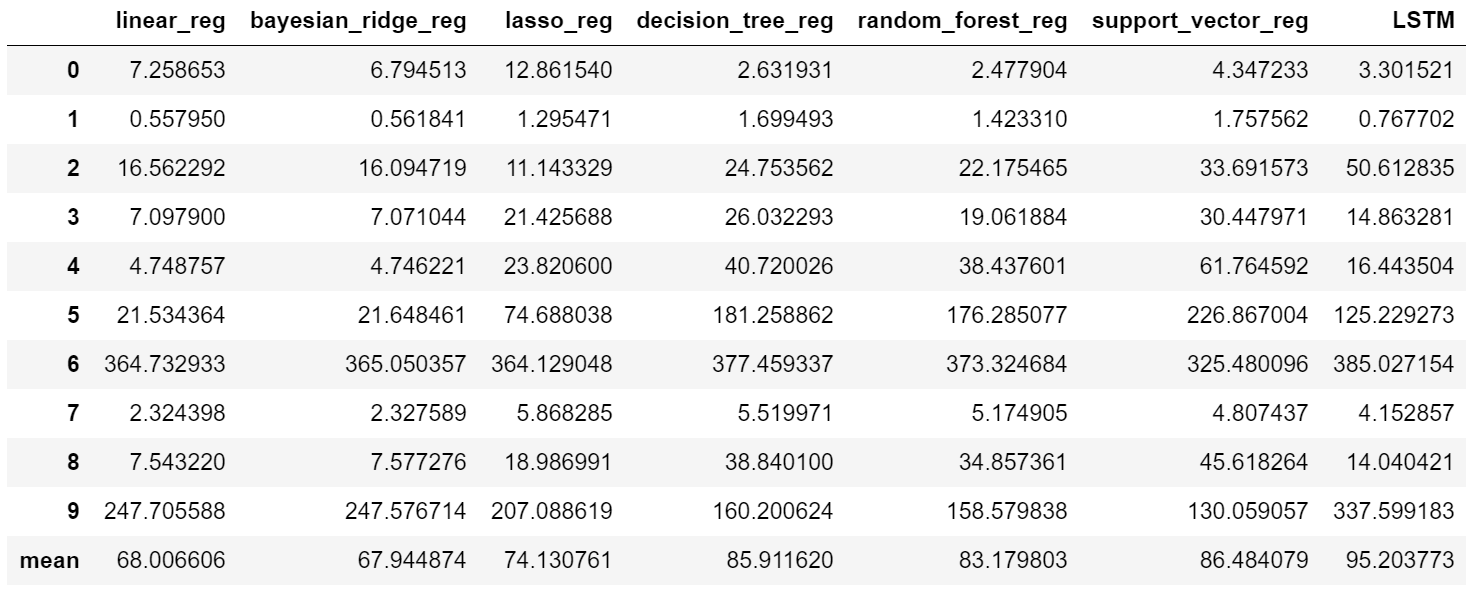
\includegraphics[width=\linewidth, height=0.12\textheight]{./image/AAPL_special_rmse.PNG}

	\caption{AAPL's RMSE values for k-fold cross validation with blocking}
	\label{figure:AAPL_special_rmse}
\end{figure}

Figure \ref{figure:RMSE_prediction}, \ref{figure:AAPL_RMSE_prediction}, and \ref{figure:JNJ_RMSE_prediction} show the daily open stock price forecast plots for the seven machine learning models on the most recent k-fold splits for IBM, AAPL, and JNJ stocks respectively.

\begin{figure}
	\subfigure[Linear Regression]{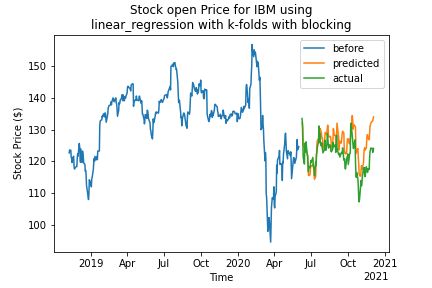
\includegraphics[width=\linewidth, height=0.12\textheight]{./image/result/IBM_open_price_forcast_using_linear_regression_with_blocking.png}}
	\subfigure[Bayesian Ridge Regression]{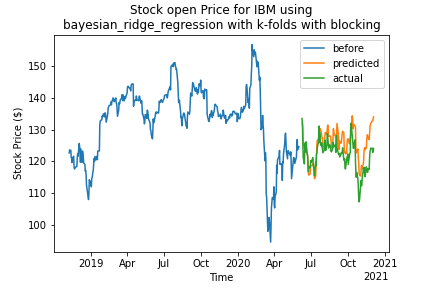
\includegraphics[width=\linewidth, height=0.12\textheight]{./image/result/IBM_open_price_forcast_using_bayesian_ridge_regression_with_blocking.png}}
	\subfigure[Lasso Regression]{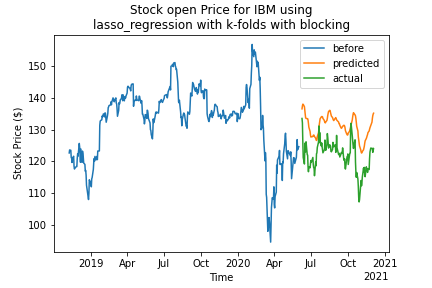
\includegraphics[width=\linewidth, height=0.12\textheight]{./image/result/IBM_open_price_forcast_using_lasso_regression_with_blocking.png}}
	\subfigure[Decision Tree Regression]{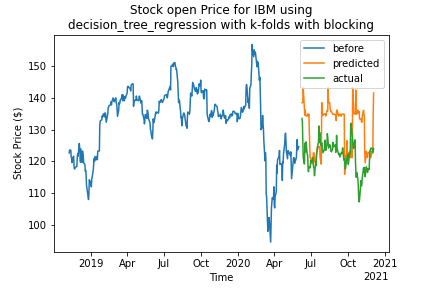
\includegraphics[width=\linewidth, height=0.12\textheight]{./image/result/IBM_open_price_forcast_using_decision_tree_regression_with_blocking.png}}
	\subfigure[Random Forest Regression]{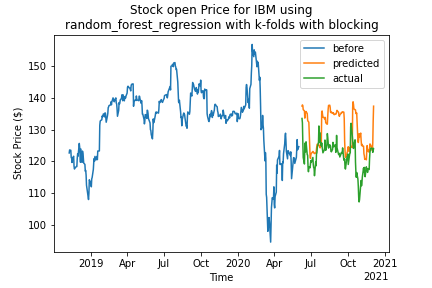
\includegraphics[width=\linewidth, height=0.12\textheight]{./image/result/IBM_open_price_forcast_using_random_forest_regression_with_blocking.png}}
	\subfigure[Support Vector Regression]{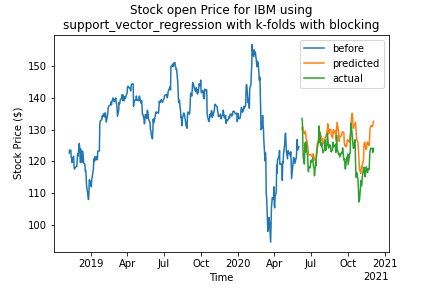
\includegraphics[width=\linewidth, height=0.12\textheight]{./image/result/IBM_open_price_forcast_using_support_vector_regression_with_blocking.png}}
	\subfigure[Long Short Term Memory]{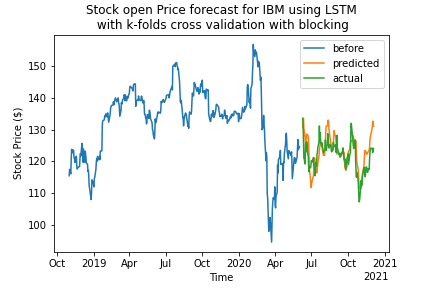
\includegraphics[width=\linewidth, height=0.12\textheight]{./image/result/IBM_open_price_forcast_using_LSTM_k_fold_with_blocking.png}}
	\caption{IBM stock price prediction with seven different machine learning models)}
	\label{figure:RMSE_prediction}
\end{figure}

\begin{figure}
	\subfigure[Linear Regression]{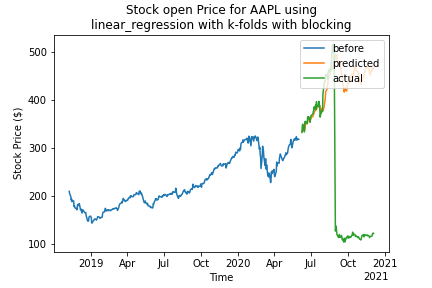
\includegraphics[width=\linewidth, height=0.12\textheight]{./image/result/AAPL_open_price_forcast_using_linear_regression_with_blocking.png}}
	\subfigure[Bayesian Ridge Regression]{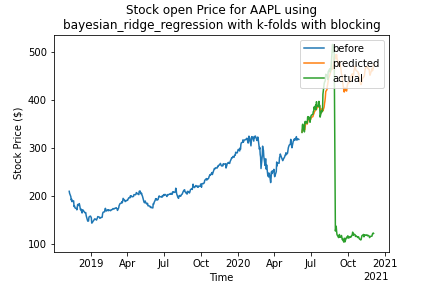
\includegraphics[width=\linewidth, height=0.12\textheight]{./image/result/AAPL_open_price_forcast_using_bayesian_ridge_regression_with_blocking.png}}
	\subfigure[Lasso Regression]{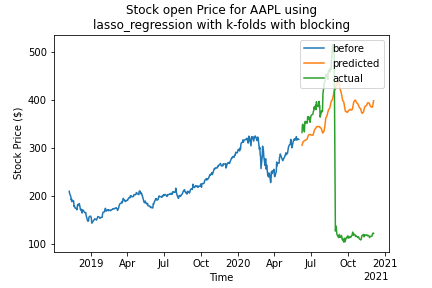
\includegraphics[width=\linewidth, height=0.12\textheight]{./image/result/AAPL_open_price_forcast_using_lasso_regression_with_blocking.png}}
	\subfigure[Decision Tree Regression]{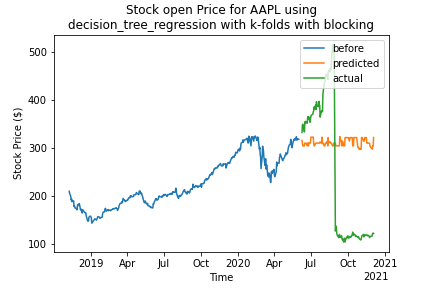
\includegraphics[width=\linewidth, height=0.12\textheight]{./image/result/AAPL_open_price_forcast_using_decision_tree_regression_with_blocking.png}}
	\subfigure[Random Forest Regression]{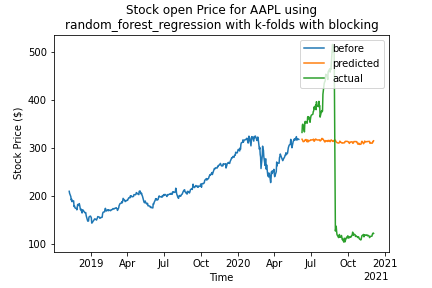
\includegraphics[width=\linewidth, height=0.12\textheight]{./image/result/AAPL_open_price_forcast_using_random_forest_regression_with_blocking.png}}
	\subfigure[Support Vector Regression]{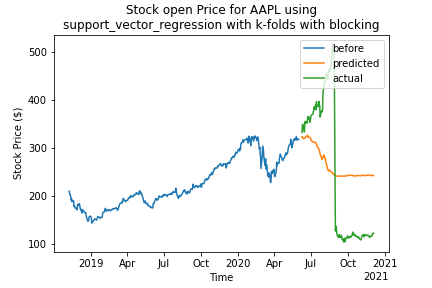
\includegraphics[width=\linewidth, height=0.12\textheight]{./image/result/AAPL_open_price_forcast_using_support_vector_regression_with_blocking.png}}
	\subfigure[Long Short Term Memory]{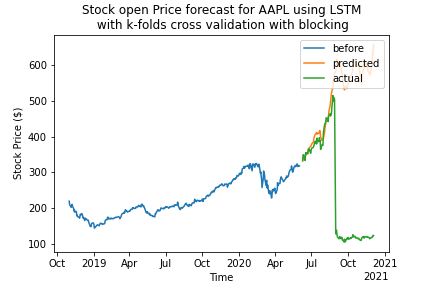
\includegraphics[width=\linewidth, height=0.12\textheight]{./image/result/AAPL_open_price_forcast_using_LSTM_k_fold_with_blocking.png}}
	\caption{AAPL stock price prediction with seven different machine learning models)}
	\label{figure:AAPL_RMSE_prediction}
\end{figure}

\begin{figure}
	\subfigure[Linear Regression]{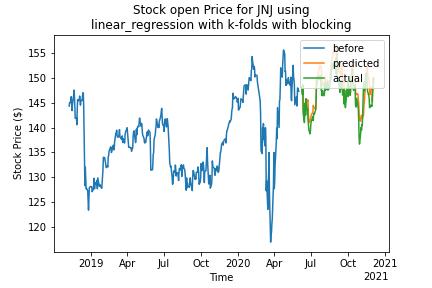
\includegraphics[width=\linewidth, height=0.12\textheight]{./image/result/JNJ_open_price_forcast_using_linear_regression_with_blocking.png}}
	\subfigure[Bayesian Ridge Regression]{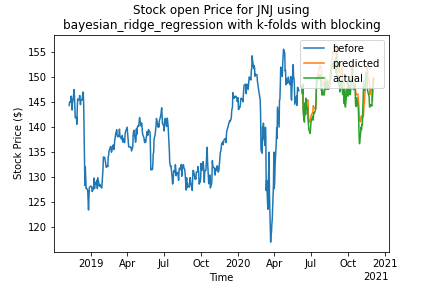
\includegraphics[width=\linewidth, height=0.12\textheight]{./image/result/JNJ_open_price_forcast_using_bayesian_ridge_regression_with_blocking.png}}
	\subfigure[Lasso Regression]{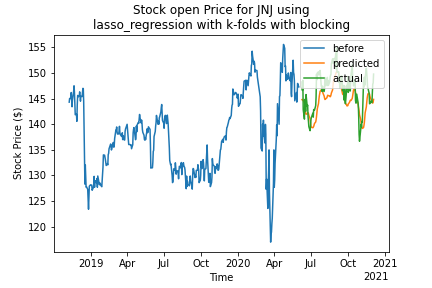
\includegraphics[width=\linewidth, height=0.12\textheight]{./image/result/JNJ_open_price_forcast_using_lasso_regression_with_blocking.png}}
	\subfigure[Decision Tree Regression]{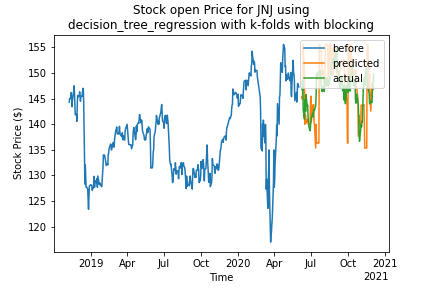
\includegraphics[width=\linewidth, height=0.12\textheight]{./image/result/JNJ_open_price_forcast_using_decision_tree_regression_with_blocking.png}}
	\subfigure[Random Forest Regression]{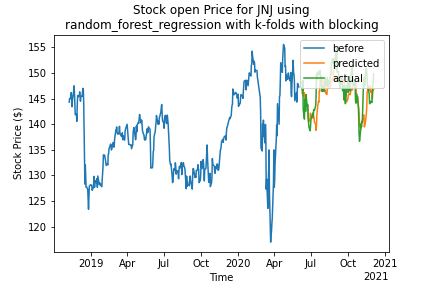
\includegraphics[width=\linewidth, height=0.12\textheight]{./image/result/JNJ_open_price_forcast_using_random_forest_regression_with_blocking.png}}
	\subfigure[Support Vector Regression]{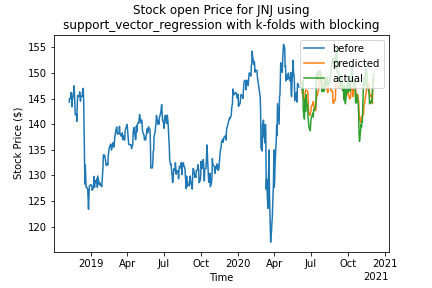
\includegraphics[width=\linewidth, height=0.12\textheight]{./image/result/JNJ_open_price_forcast_using_support_vector_regression_with_blocking.png}}
	\subfigure[Long Short Term Memory]{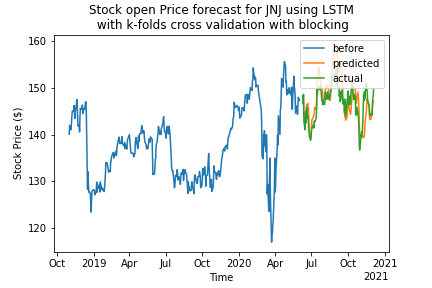
\includegraphics[width=\linewidth, height=0.12\textheight]{./image/result/JNJ_open_price_forcast_using_LSTM_k_fold_with_blocking.png}}
	\caption{JNJ stock price prediction with seven different machine learning models)}
	\label{figure:JNJ_RMSE_prediction}
\end{figure}


\section{Conclusion and Future Works}

Daily stock price are predicted by applying machine learning models to past 5 days' technical indicators, that consists of the volume of trade, dividend, simple moving average (SMA), exponential moving average (EMA), moving average convergence/divergence (MACD), stochastic oscillator (STOCH), relative strength index (RSI), average directional movement index (ADX), commodity channel index (CCI), Aroon indicator (AROON), Bollinger bands (BBANDS), Chaikin A/D line (AD), and on balance volume (OBV). The stocks that were investigated are IBM, Apple and Johnson and Johnson. Stock price and technical indicator data for the past almost 20 years are used to train the models after pre-processing steps such as k-fold cross-validation split with blocking, normalization with standard scaler and min max scaler, as well as principle component analysis for dimensionality reduction.

From measuring the root mean square error of the prediction with the actual stock price, the best models are long short term memory model, linear regression model and Bayesian ridge regression model. For IBM stock, they all have a RMSE score of around 2 to 5 for all price types. For JNJ, even smaller RMSEs are obtained. However, this approach of predicting stocks through technical indicators do not seem to work for AAPL. All the models have a RMSEs of above 120. Therefore, this approach of stock price prediction through analyzing technical indicators might not be applicable to all kinds of stocks, but it is promising to some particular stocks that have trends more correlated with past technical indicators.

Through designing the machine learning pipeline, the effects of k-fold cross-validation with or without blocking and whether to perform PCA is studied. From results of experimentation, k-fold cross-validation with blocking shows better prediction result. This is consistent with the nature of the stock price data. As the stock market changes, the trend and correlation with technical indicator also changes. Therefore, training a model over a very long period of time by not using blocking will make the model too generalized for future predictions. The impact of PCA on prediction performance are different for each model. In general, the dimensionality reduction produces better result, but the main benefit comes from reduced computation time.

To improve on this project, the independent variable can be adjusted to price difference between next day and current day. This might improve the prediction result, as in this project, actual past stock prices are not considered during prediction. This will help to isolate the effect of original stock price. Another improvement to the project can be to obtain a multi-day forecast instead of just a next-day forecast, by continue predicting on predicted data. However, this will require calculations of technical indicators based on daily open, daily close, daily high, and daily low predicted prices. Since some features depend on volume of trade, it would require some assumption or prediction for volume of trade to obtain in order to build further predictions. One additional feature can be added before using this approach is to identify stocks that are likely to be correlated with technical indicators like the IBM and JNJ studied in this case. This will save time and computational power so it is not wasted to obtain unusable results for stocks like AAPL. One the other hand, more factors like company news and fundamental analysis of the stock can be included to make this approach more generalized for all kinds of stocks.


\section*{Bibliography}

\begin{thebibliography}{00}
\bibitem{b1} W. Jasic, “The profitability of daily stock market indices trades based on neural network predictions: case study for the S\&P 500, the DAX, the TOPIX and the FTSE in the period 1965-1999,” Applied financial economics, vol. 14, no. 4, pp. 285–297, Feb. 2004, doi: 10.1080/0960310042000201228.
\bibitem{b2} C. Yu, “Evolving Least Squares Support Vector Machines for Stock Market Trend Mining,” IEEE transactions on evolutionary computation, vol. 13, no. 1, pp. 87–102, Feb. 2009, doi: 10.1109/TEVC.2008.928176.
\bibitem{b3} D. L. Minh, A. Sadeghi-Niaraki, H. D. Huy, K. Min, H. Moon, Deep learning approach
for short-term stock trends prediction based on two-stream gated recurrent unit network,
Ieee Access 6 (2018) 55392–55404 (2018).
\bibitem{b4} W. Wang, “Stock2Vec: A Hybrid Deep Learning Framework for Stock Market Prediction with Representation Learning and Temporal Convolutional Network,” Sep. 2020.
\bibitem{b5} K. Ntakaris, “Mid-price prediction based on machine learning methods with technical and quantitative indicators,” PloS one, vol. 15, no. 6, pp. e0234107–e0234107, Jun. 2020, doi: 10.1371/journal.pone.0234107.
\bibitem{b6} J. Patel, S. Shah, P. Thakkar, and K. Kotecha, “Predicting stock and stock price index movement using Trend Deterministic Data Preparation and machine learning techniques,” Expert Systems with Applications, vol. 42, no. 1, pp. 259–268, 2015. 
\vspace{12pt}
\end{thebibliography}

\end{document}
